% sections/04_estimation.tex -- Section 4 (W1b). Plan: BLUEPRINT 2.4, 3.2 (eq:profile, eq:msm), 8.3-8.6, 9; Overrides O1, O2, O5, O6.
% Provenance convention (Override O5): "% src: <file>:<line>" follows every sentence that carries a number.
% Abbreviations in src comments: 5:NN = frot/sub2025/5_quantitative_model.tex; 11:NN = 11_app_data.tex; 12:NN = 12_app_quant.tex;
% T: = paper/tables/; F: = paper/figures/abdou/ (embedded data rows, age in the first column); D0N = dossier/0N_*.md; QJE:NN = rendered May 2025 text.
% Vintage rule (BLUEPRINT Decision 8): point estimates identical in both vintages; standard errors and chi-square from the 2026 file
% T:estimated_parameters.tex (footnoted in Table 3); fit series from the 2026 files F:h800_*_edit_c.tex (footnoted in Figure 2 and B1).
\section{Data, Estimation, and Fit}\label{sec:estimation}

The model is estimated in two steps, as in \citet{Cagetti2003} and \citet{Gourinchas2002}. % src: 5:371-373
The first step estimates from the data, or takes from program rules and the literature, every input that does not require solving the model: health transitions, survival, medical spending, wage profiles and the ability process, the initial distribution at age 30, and the institutional parameters of \autoref{sec:institutions}. The second step estimates the seven preference parameters by the method of simulated moments (MSM), taking the first-step inputs as given. % src: 5:373-379; 5:533
\autoref{subsec:gradient} collects the differences by health in the data profiles on which the reforms of \autoref{sec:elimination} to \autoref{sec:other} act; \autoref{app:data} and \autoref{app:estimation} give the details.

\subsection{Data and samples}\label{subsec:data}

The primary data source is the Panel Study of Income Dynamics (PSID), the longitudinal survey of US families conducted by the Survey Research Center at the University of Michigan since 1968, with interviews every year until 1997 and every two years thereafter.\footnote{Panel Study of Income Dynamics, public use dataset, produced and distributed by the Survey Research Center, Institute for Social Research, University of Michigan, \url{https://psidonline.isr.umich.edu/}.} % src: 11:14
We use the 1968--2015 waves and the Survey Research Center component of the original sample, and we keep household heads and spouses born between 1920 and 1940, a cohort that faced similar Social Security rules and whose outcomes the PSID records across the life cycle. % src: 11:16; 11:18; T:sample_psid.tex:10,13
The sample has 2,248 individuals and 44,404 person-year observations (\autoref{tab:psid}). % src: T:sample_psid.tex:13; 11:51
It provides the health transitions, survival probabilities, wage profiles and wage dynamics, the initial distribution of state variables, and the labor supply and asset profiles that the model is estimated to match. % src: 11:51
Medical spending and insurance coverage come from the Medical Expenditure Panel Survey (MEPS) of the Agency for Healthcare Research and Quality, in which spending reported by individuals is cross-validated with medical providers and insurers.\footnote{Medical Expenditure Panel Survey, Agency for Healthcare Research and Quality, \url{https://meps.ahrq.gov/}.} % src: 11:58
We use the 1999--2012 waves and keep household heads aged 20 and older with nonmissing age, medical spending, insurance coverage during working ages, and health status: 120,731 individuals and 211,709 person-year observations (\autoref{tab:meps}). % src: 11:60; T:sample_meps.tex:16
All monetary values in the paper are in 2016 dollars, except the statutory Social Security parameters of \autoref{tab:ssparams}, which are in 1987 dollars. % src: 5:620; 11:177; 12:36

Health is measured in the PSID from three work-limitation questions asked in every wave, following \citet{Low2015}. Good health ($h=0$) is no condition that limits work, and poor health ($h=1$) is a condition that limits work somewhat or just a little. A disability ($h=2$) is a condition that keeps the respondent from doing any type of work and limits the amount of work a lot, the criterion of the Social Security Administration for disability insurance. % src: 11:92-98
In the MEPS, health is classified from self-rated health in the three interviews of a year, following \citet{Pashchenko2019}: a disability is a rating of poor in any interview, good health a rating of good or better in all three, and poor health the remainder. % src: 11:100-102
The two measures give similar shares with a disability by age band---9.3 percent in the PSID and 10 percent in the MEPS at ages 50--60, 12.9 and 11.7 percent at ages 60--70---while the MEPS classifies more individuals as being in poor health (\autoref{tab:health}). % src: T:health_measures.tex:16-17
\autoref{app:data} reproduces the survey items.

\subsection{First step: profiles by health}\label{subsec:firststep}

Health transitions are probit regressions of the indicator of next year's health state on age dummies, estimated on the subsample in each current state, with the predicted probabilities interpolated linearly across ages. % src: 11:133-134
Survival is a logit of an indicator of survival on a quadratic in age, lagged health, and their interaction, estimated on 132,070 PSID person-years (\autoref{tab:survival}). % src: 11:139; T:survival_coeffs.tex:10-16
Out-of-pocket medical spending is total spending times one minus the coverage share, both estimated on age and year dummies by health group in the MEPS following \citet{Pashchenko2019}, with coverage from private insurance before age 65 and from Medicare afterward. The profiles are multiplied by 1.60 before age 65 and by 1.90 from age 65 to match the National Health Expenditure Accounts, following \citet{Denardi2018}, and smoothed on a quadratic in age. % src: 11:167-171
Hourly wages are annual earnings divided by annual hours in the PSID, trimmed below \$6.50 and above \$250, and corrected for selection into work with the two-stage procedure of \citet{Heckman1976} as applied by \citet{Guner2012}, in which log wages are regressed on age polynomials, their interactions with health, and the inverse Mills ratio from a participation probit, on 64,941 observations (\autoref{tab:wages}). % src: 11:177-182; T:wages_coeffs.tex:15-63
The persistence and innovation variance of ability in \eqref{eq:wage} are estimated by maximum likelihood with the Kalman filter on the wage residuals at ages 25--65, dropping the top 0.5 percent of residuals; the estimates are $(\rho,\sigma_\varepsilon^2)=(0.981,\,0.016)$. % src: 11:188-190
The initial distribution at age 30 is the empirical joint distribution of wages, health, assets, and participation of sample members aged 28--32, with the mean of log wages adjusted to the estimated profile within each health group, and with average indexed earnings imputed from five years of work at 2,000 hours a year at the age-30 wage, following \citet{french2005effects} (\autoref{tab:initial}). % src: 11:222

\autoref{fig:firststep} shows the four first-step profiles by health. The probability of remaining in good health falls with age, and the decline is absorbed mainly by transitions into poor health. % src: F:frot_disab0_edit.tex
Mortality rises with age for every health state and fastest, at older ages, for individuals with a disability. % src: F:frot_mortal7_edit2.tex; 5:507-509
Out-of-pocket medical spending rises with age and is ordered by health at every age, highest for individuals with a disability. % src: F:frot_oopmedical_2016_edit.tex; 5:511-513
Hourly wages are hump-shaped in age for every health state and are ordered the other way: healthy workers earn more than workers in poor health, who earn more than workers with a disability. % src: F:frot_wageselection_n800_edit.tex; 5:516
\autoref{subsec:gradient} reports the values at the ages that matter for the reforms.

\begin{figure}[!tp]
\centering
\caption{First-Step Profiles by Health Status}
\label{fig:firststep}
\vspace{6pt}
\begin{tabular}{cc}
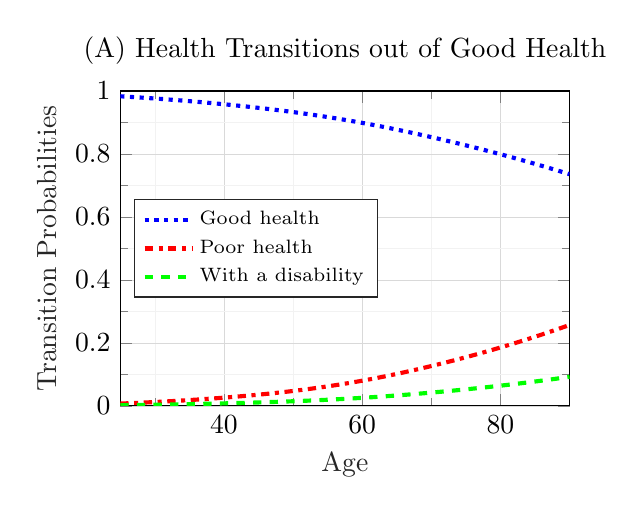
\begin{tikzpicture}
\begin{axis}[%
width=5.706cm,
height=4cm,
at={(0cm,0cm)},
scale only axis,
xmin=25,
xmax=90,
xlabel style={font=\color{white!15!black}},
xlabel={Age},
ymin=0,
ymax=1,
ylabel style={font=\color{white!15!black}},
ylabel={Transition Probabilities},
axis background/.style={fill=white},
%title style={font=\bfseries},
title={(A) Health Transitions out of Good Health},
legend style={at={(0.03,0.5)}, anchor=west, legend cell align=left, align=left, draw=white!15!black,font=\scriptsize},
grid=both,
grid style={line width=0.2pt, draw=gray!30},
minor grid style={line width=0.1pt, draw=gray!10},
minor tick num=1
]
% Blue line - h(t)=0 - dotted line
\addplot [color=blue, line width=1.5pt, dotted]
  table[row sep=crcr]{%
25 0.98309247\\
26 0.98177065\\
27 0.98040043\\
28 0.97898087\\
29 0.97751107\\
30 0.97599011\\
31 0.97441706\\
32 0.97279099\\
33 0.97111097\\
34 0.96937609\\
35 0.96758542\\
36 0.96573805\\
37 0.96383308\\
38 0.96186959\\
39 0.95984659\\
40 0.95776298\\
41 0.95561743\\
42 0.95340817\\
43 0.95113281\\
44 0.94878801\\
45 0.94636924\\
46 0.94387079\\
47 0.94128627\\
48 0.93861018\\
49 0.93583981\\
50 0.93297328\\
51 0.93000876\\
52 0.92694444\\
53 0.92377856\\
54 0.92050939\\
55 0.91713528\\
56 0.91365461\\
57 0.91006583\\
58 0.90636744\\
59 0.90255801\\
60 0.89863619\\
61 0.89460071\\
62 0.89045035\\
63 0.88618399\\
64 0.88180192\\
65 0.87730914\\
66 0.87271271\\
67 0.86801917\\
68 0.86323358\\
69 0.85835934\\
70 0.85339844\\
71 0.84835184\\
72 0.8432198\\
73 0.83800218\\
74 0.83269856\\
75 0.82730842\\
76 0.82183118\\
77 0.81626625\\
78 0.81061306\\
79 0.80487101\\
80 0.79903956\\
81 0.79311816\\
82 0.78710628\\
83 0.78100339\\
84 0.77480897\\
85 0.76852255\\
86 0.76214369\\
87 0.75567204\\
88 0.74910741\\
89 0.74244985\\
90 0.73569986\\
};
\addlegendentry{Good health}

% Red line - h(t)=1 - dash-dotted line
\addplot [color=red, line width=1.5pt, dashdotted]
  table[row sep=crcr]{%
25 0.00740989\\
26 0.00829385\\
27 0.0092242\\
28 0.01020239\\
29 0.01122993\\
30 0.01230832\\
31 0.01343908\\
32 0.01462377\\
33 0.01586393\\
34 0.01716114\\
35 0.01851696\\
36 0.01993295\\
37 0.02141069\\
38 0.02295175\\
39 0.02455777\\
40 0.02623054\\
41 0.02797205\\
42 0.02978474\\
43 0.03167175\\
44 0.0336372\\
45 0.03568655\\
46 0.03782661\\
47 0.04006511\\
48 0.04240901\\
49 0.04486246\\
50 0.04742877\\
51 0.05011122\\
52 0.05291311\\
53 0.05583768\\
54 0.05888815\\
55 0.0620677\\
56 0.06537945\\
57 0.06882647\\
58 0.07241176\\
59 0.07613823\\
60 0.08000872\\
61 0.08402595\\
62 0.08819256\\
63 0.09251107\\
64 0.09698204\\
65 0.10159943\\
66 0.10635428\\
67 0.1112381\\
68 0.11624445\\
69 0.12136908\\
70 0.1266097\\
71 0.13196542\\
72 0.13743634\\
73 0.14302316\\
74 0.14872693\\
75 0.15454888\\
76 0.16049033\\
77 0.16655263\\
78 0.1727371\\
79 0.17904508\\
80 0.18547785\\
81 0.1920367\\
82 0.19872287\\
83 0.20553761\\
84 0.21248211\\
85 0.21955753\\
86 0.22676493\\
87 0.23410525\\
88 0.24157916\\
89 0.24918697\\
90 0.25692832\\
};
\addlegendentry{Poor health}

% Green line - h(t)=2 - dashed line
\addplot [color=green, line width=1.5pt, dashed]
  table[row sep=crcr]{%
25 0.00232342\\
26 0.00258882\\
27 0.00286849\\
28 0.00316296\\
29 0.00347276\\
30 0.00379847\\
31 0.00414063\\
32 0.00449986\\
33 0.00487673\\
34 0.00527188\\
35 0.00568592\\
36 0.00611948\\
37 0.00657321\\
38 0.00704778\\
39 0.00754387\\
40 0.00806223\\
41 0.0086037\\
42 0.00916924\\
43 0.00976009\\
44 0.0103778\\
45 0.01102439\\
46 0.01170237\\
47 0.0124146\\
48 0.01316373\\
49 0.01395159\\
50 0.01477974\\
51 0.0156498\\
52 0.01656341\\
53 0.01752226\\
54 0.01852807\\
55 0.01958259\\
56 0.02068762\\
57 0.02184496\\
58 0.02305648\\
59 0.02432406\\
60 0.02564961\\
61 0.02703505\\
62 0.02848236\\
63 0.02999351\\
64 0.03156963\\
65 0.03320868\\
66 0.03490704\\
67 0.03666119\\
68 0.03846841\\
69 0.040327\\
70 0.04223612\\
71 0.04419564\\
72 0.04620591\\
73 0.04826763\\
74 0.05038168\\
75 0.05254912\\
76 0.05477106\\
77 0.0570487\\
78 0.05938328\\
79 0.06177607\\
80 0.0642284\\
81 0.06674166\\
82 0.06931726\\
83 0.07195667\\
84 0.07466143\\
85 0.07743309\\
86 0.08027324\\
87 0.08318347\\
88 0.08616529\\
89 0.08922008\\
90 0.0923489\\
};
\addlegendentry{With a disability}
\end{axis}
\end{tikzpicture} & 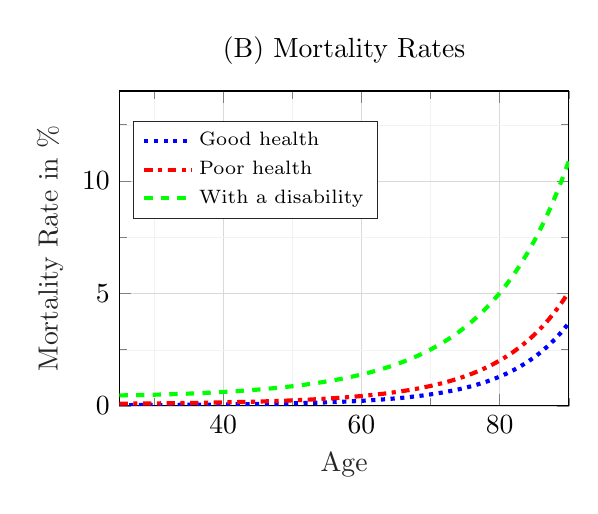
\begin{tikzpicture}
\begin{axis}[%
width=5.706cm,
height=4cm,
at={(0cm,0cm)},
scale only axis,
xmin=25,
xmax=90,
xlabel style={font=\color{white!15!black}},
xlabel={Age},
ymin=0,
ymax=14,
ylabel style={font=\color{white!15!black}},
ylabel={Mortality Rate in \%},
axis background/.style={fill=white},
%title style={font=\bfseries},
title={(B) Mortality Rates},
legend style={at={(axis cs:27,10.5)}, anchor=west, legend cell align=left, align=left, draw=white!15!black, font=\scriptsize},
grid=both,
grid style={line width=0.2pt, draw=gray!30},
minor grid style={line width=0.1pt, draw=gray!10},
minor tick num=1
]
% Back line (Overall) - full
% \addplot [color=black, line width=1.5pt]
%   table[row sep=crcr]{%
% 25 0.04479\\
% 26 0.04675\\
% 27 0.0481\\
% 28 0.05082\\
% 29 0.05277\\
% 30 0.05375\\
% 31 0.05639\\
% 32 0.05905\\
% 33 0.06249\\
% 34 0.06579\\
% 35 0.06926\\
% 36 0.07637\\
% 37 0.07822\\
% 38 0.08325\\
% 39 0.08796\\
% 40 0.09379\\
% 41 0.09919\\
% 42 0.10925\\
% 43 0.11504\\
% 44 0.12074\\
% 45 0.12909\\
% 46 0.13868\\
% 47 0.1475\\
% 48 0.15626\\
% 49 0.16962\\
% 50 0.18554\\
% 51 0.20082\\
% 52 0.21588\\
% 53 0.23697\\
% 54 0.25106\\
% 55 0.27595\\
% 56 0.30314\\
% 57 0.32832\\
% 58 0.35589\\
% 59 0.38782\\
% 60 0.41329\\
% 61 0.45229\\
% 62 0.48501\\
% 63 0.52826\\
% 64 0.55276\\
% 65 0.59562\\
% 66 0.66072\\
% 67 0.70075\\
% 68 0.74535\\
% 69 0.80985\\
% 70 0.87603\\
% 71 1.00144\\
% 72 1.03708\\
% 73 1.21095\\
% 74 1.28609\\
% 75 1.47924\\
% 76 1.53636\\
% 77 1.74536\\
% 78 1.86332\\
% 79 2.00865\\
% 80 2.31624\\
% 81 2.51996\\
% 82 2.79552\\
% 83 3.17659\\
% 84 3.35743\\
% 85 3.97544\\
% 86 4.09512\\
% 87 4.87983\\
% 88 5.39166\\
% 89 6.00628\\
% 90 6.48326\\
% };
% \addlegendentry{Overall}
% Blue line (Good health) - dotted
\addplot [color=blue, line width=1.5pt, dotted]
  table[row sep=crcr]{%
25 0.035\\
26 0.03614\\
27 0.03736\\
28 0.03868\\
29 0.04009\\
30 0.0416\\
31 0.04323\\
32 0.04497\\
33 0.04685\\
34 0.04886\\
35 0.05103\\
36 0.05335\\
37 0.05586\\
38 0.05855\\
39 0.06146\\
40 0.06458\\
41 0.06795\\
42 0.07159\\
43 0.07552\\
44 0.07975\\
45 0.08434\\
46 0.0893\\
47 0.09467\\
48 0.10049\\
49 0.1068\\
50 0.11365\\
51 0.12109\\
52 0.12917\\
53 0.13798\\
54 0.14756\\
55 0.158\\
56 0.1694\\
57 0.18184\\
58 0.19545\\
59 0.21032\\
60 0.22662\\
61 0.24448\\
62 0.26407\\
63 0.28558\\
64 0.30923\\
65 0.33525\\
66 0.3639\\
67 0.39548\\
68 0.43033\\
69 0.46882\\
70 0.51137\\
71 0.55844\\
72 0.61059\\
73 0.66839\\
74 0.73254\\
75 0.80378\\
76 0.88297\\
77 0.97108\\
78 1.06919\\
79 1.17854\\
80 1.3005\\
81 1.43664\\
82 1.58871\\
83 1.75871\\
84 1.94885\\
85 2.16166\\
86 2.39997\\
87 2.66694\\
88 2.96613\\
89 3.30152\\
90 3.67755\\
};
\addlegendentry{Good health}

% Red line (Poor health) - dash-dotted
\addplot [color=red, line width=1.5pt, dashdotted]
  table[row sep=crcr]{%
25 0.09962\\
26 0.10175\\
27 0.10405\\
28 0.10654\\
29 0.10922\\
30 0.11212\\
31 0.11523\\
32 0.11858\\
33 0.12218\\
34 0.12605\\
35 0.1302\\
36 0.13466\\
37 0.13944\\
38 0.14458\\
39 0.15009\\
40 0.15601\\
41 0.16236\\
42 0.16919\\
43 0.17652\\
44 0.18441\\
45 0.19288\\
46 0.202\\
47 0.21181\\
48 0.22237\\
49 0.23376\\
50 0.24603\\
51 0.25927\\
52 0.27356\\
53 0.289\\
54 0.30569\\
55 0.32375\\
56 0.3433\\
57 0.36448\\
58 0.38745\\
59 0.41237\\
60 0.43943\\
61 0.46884\\
62 0.50084\\
63 0.53568\\
64 0.57364\\
65 0.61503\\
66 0.66022\\
67 0.70958\\
68 0.76354\\
69 0.82259\\
70 0.88726\\
71 0.95816\\
72 1.03592\\
73 1.12131\\
74 1.21513\\
75 1.31831\\
76 1.43187\\
77 1.55694\\
78 1.6948\\
79 1.84687\\
80 2.01472\\
81 2.20011\\
82 2.40499\\
83 2.63155\\
84 2.8822\\
85 3.15962\\
86 3.46679\\
87 3.80701\\
88 4.1839\\
89 4.60146\\
90 5.06408\\
};
\addlegendentry{Poor health}

% Green line (With a Disability) - dashed
\addplot [color=green, line width=1.5pt, dashed]
  table[row sep=crcr]{%
25 0.46695\\
26 0.47172\\
27 0.47714\\
28 0.48322\\
29 0.48999\\
30 0.49748\\
31 0.50572\\
32 0.51473\\
33 0.52456\\
34 0.53524\\
35 0.54682\\
36 0.55934\\
37 0.57287\\
38 0.58745\\
39 0.60316\\
40 0.62006\\
41 0.63821\\
42 0.65772\\
43 0.67867\\
44 0.70115\\
45 0.72527\\
46 0.75115\\
47 0.77892\\
48 0.8087\\
49 0.84066\\
50 0.87496\\
51 0.91177\\
52 0.9513\\
53 0.99376\\
54 1.03937\\
55 1.0884\\
56 1.14113\\
57 1.19786\\
58 1.25892\\
59 1.32469\\
60 1.39555\\
61 1.47196\\
62 1.55439\\
63 1.64337\\
64 1.73947\\
65 1.84333\\
66 1.95565\\
67 2.07718\\
68 2.20877\\
69 2.35133\\
70 2.50586\\
71 2.67347\\
72 2.85536\\
73 3.05287\\
74 3.26744\\
75 3.50067\\
76 3.75428\\
77 4.03018\\
78 4.33044\\
79 4.65732\\
80 5.01328\\
81 5.40098\\
82 5.82331\\
83 6.28341\\
84 6.78464\\
85 7.33061\\
86 7.92519\\
87 8.57248\\
88 9.27686\\
89 10.04289\\
90 10.87536\\
};
\addlegendentry{With a disability}
\end{axis}
\end{tikzpicture}\\[1.5ex]
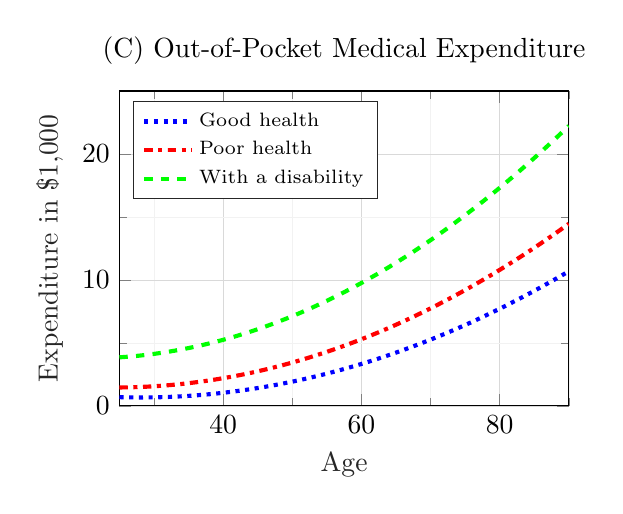
\begin{tikzpicture}
\begin{axis}[%
width=5.706cm,
height=4cm,
at={(0cm,0cm)},
scale only axis,
xmin=25,
xmax=90,
xlabel style={font=\color{white!15!black}},
xlabel={Age},
ymin=0,
ymax=25,
ylabel style={font=\color{white!15!black}},
ylabel={Expenditure in \$1,000},
axis background/.style={fill=white},
%title style={font=\bfseries},
title={(C) Out-of-Pocket Medical Expenditure},
legend style={at={(axis cs:27,20.3)}, anchor=west, legend cell align=left, align=left, draw=white!15!black, font=\scriptsize},
grid=both,
grid style={line width=0.2pt, draw=gray!30},
minor grid style={line width=0.1pt, draw=gray!10},
minor tick num=1
]
% Blue line (h(t)=0) - dotted
\addplot [color=blue, line width=1.5pt, dotted]
  table[row sep=crcr]{%
25 0.69549069\\
26 0.68199083\\
27 0.67371464\\
28 0.6706623\\
29 0.67283363\\
30 0.68022881\\
31 0.69284784\\
32 0.71069035\\
33 0.73375671\\
34 0.76204674\\
35 0.79556062\\
36 0.83429816\\
37 0.87825956\\
38 0.92744462\\
39 0.98185335\\
40 1.04148593\\
41 1.10634236\\
42 1.17642228\\
43 1.25172585\\
44 1.33225347\\
45 1.41800457\\
46 1.5089797\\
47 1.60517831\\
48 1.70660078\\
49 1.81324709\\
50 1.92511801\\
51 2.04221129\\
52 2.16452841\\
53 2.29206939\\
54 2.42483423\\
55 2.56282291\\
56 2.70603545\\
57 2.85447183\\
58 3.00813021\\
59 3.1670143\\
60 3.33112225\\
61 3.50045404\\
62 3.67500783\\
63 3.85478546\\
64 4.03978882\\
65 4.23001602\\
66 4.42546521\\
67 4.62613826\\
68 4.83203516\\
69 5.0431559\\
70 5.25950051\\
71 5.48107082\\
72 5.70786313\\
73 5.93987742\\
74 6.17711743\\
75 6.41958129\\
76 6.667269\\
77 6.92017871\\
78 7.17831412\\
79 7.44167339\\
80 7.71025465\\
81 7.98406162\\
82 8.26309058\\
83 8.5473434\\
84 8.83682006\\
85 9.13152245\\
86 9.43144682\\
87 9.73659504\\
88 10.0469652\\
89 10.362563\\
90 10.6833828\\
};
\addlegendentry{Good health}

% Red line (h(t)=1) - dash-dotted
\addplot [color=red, line width=1.5pt, dashdotted]
  table[row sep=crcr]{%
25 1.46408419\\
26 1.47088973\\
27 1.48372673\\
28 1.50259464\\
29 1.52749401\\
30 1.55842446\\
31 1.59538601\\
32 1.63837884\\
33 1.68740294\\
34 1.74245794\\
35 1.8035444\\
36 1.87066252\\
37 1.94381135\\
38 2.02299071\\
39 2.10820247\\
40 2.19944476\\
41 2.29671758\\
42 2.40002279\\
43 2.50935854\\
44 2.62472481\\
45 2.74612348\\
46 2.87355268\\
47 3.00701427\\
48 3.14650454\\
49 3.29202905\\
50 3.44358224\\
51 3.60116782\\
52 3.76478393\\
53 3.93443244\\
54 4.11011148\\
55 4.29182105\\
56 4.47956301\\
57 4.6733355\\
58 4.87313852\\
59 5.07897394\\
60 5.29083989\\
61 5.50873637\\
62 5.73266525\\
63 5.96262465\\
64 6.19861645\\
65 6.44063878\\
66 6.68869164\\
67 6.94277503\\
68 7.20289082\\
69 7.46903714\\
70 7.74121585\\
71 8.01942509\\
72 8.30366486\\
73 8.59393703\\
74 8.89023973\\
75 9.19257296\\
76 9.50093858\\
77 9.81533473\\
78 10.1357614\\
79 10.4622205\\
80 10.7947101\\
81 11.1332302\\
82 11.4777846\\
83 11.8283658\\
84 12.1849813\\
85 12.5476292\\
86 12.9163038\\
87 13.2910127\\
88 13.6717522\\
89 14.0585203\\
90 14.4513245\\
};
\addlegendentry{Poor health}

% Green line (h(t)=2) - dashed
\addplot [color=green, line width=1.5pt, dashed]
  table[row sep=crcr]{%
25 3.85542075\\
26 3.89487722\\
27 3.94193474\\
28 3.99658957\\
29 4.05884358\\
30 4.12869677\\
31 4.20614726\\
32 4.29119694\\
33 4.38384579\\
34 4.48409196\\
35 4.5919373\\
36 4.70738183\\
37 4.83042552\\
38 4.9610684\\
39 5.09930859\\
40 5.24514795\\
41 5.3985865\\
42 5.55962235\\
43 5.72825925\\
44 5.90449346\\
45 6.08832499\\
46 6.27975755\\
47 6.47878743\\
48 6.68541649\\
49 6.89964472\\
50 7.12147213\\
51 7.35089685\\
52 7.58792075\\
53 7.83254383\\
54 8.08476422\\
55 8.34458379\\
56 8.61200254\\
57 8.88702046\\
58 9.16963756\\
59 9.45985011\\
60 9.7576637\\
61 10.0630765\\
62 10.3760884\\
63 10.6966977\\
64 11.0249061\\
65 11.3607119\\
66 11.7041168\\
67 12.0551246\\
68 12.4137279\\
69 12.7799285\\
70 13.1537301\\
71 13.5351272\\
72 13.9241253\\
73 14.3207226\\
74 14.7249191\\
75 15.1367111\\
76 15.5561059\\
77 15.983098\\
78 16.4176856\\
79 16.8598761\\
80 17.3096621\\
81 17.7670491\\
82 18.2320353\\
83 18.7046132\\
84 19.1848014\\
85 19.6725907\\
86 20.1679624\\
87 20.6709351\\
88 21.1815089\\
89 21.6997024\\
90 22.2254782\\
};
\addlegendentry{With a disability}
\end{axis}
\end{tikzpicture} & 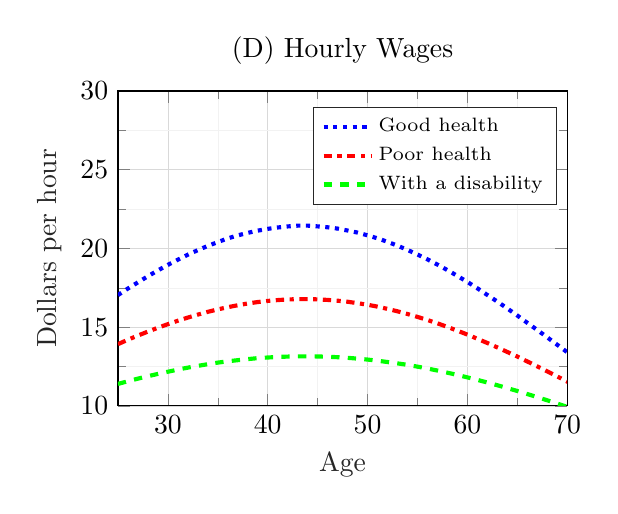
\begin{tikzpicture}
\begin{axis}[%
width=5.706cm,
height=4cm,
at={(0cm,0cm)},
scale only axis,
xmin=25,
xmax=70,
xlabel style={font=\color{white!15!black}},
xlabel={Age},
ymin=10,
ymax=30,
ylabel style={font=\color{white!15!black}},
ylabel={Dollars per hour},
axis background/.style={fill=white},
%title style={font=\bfseries},
title={(D) Hourly Wages},
legend style={at={(axis cs:69,29)}, anchor=north east, legend cell align=left, align=left, draw=white!15!black, font=\scriptsize},
grid=both,
grid style={line width=0.2pt, draw=gray!30},
minor grid style={line width=0.1pt, draw=gray!10},
minor tick num=1
]
% Blue line (h(t)=0) - dotted
\addplot [color=blue, line width=1.5pt, dotted]
  table[row sep=crcr]{%
25 17.038732931\\
26 17.4542862\\
27 17.8458896\\
28 18.2333825\\
29 18.6034326\\
30 18.9545214\\
31 19.2874174\\
32 19.6000282\\
33 19.8910738\\
34 20.1595058\\
35 20.4032752\\
36 20.6349778\\
37 20.8299873\\
38 20.9875306\\
39 21.1294096\\
40 21.2430726\\
41 21.3293168\\
42 21.3971419\\
43 21.4465891\\
44 21.4472714\\
45 21.4000386\\
46 21.3431199\\
47 21.2595208\\
48 21.1359871\\
49 21.0057627\\
50 20.8289922\\
51 20.6396637\\
52 20.4187952\\
53 20.1755905\\
54 19.9054845\\
55 19.6151301\\
56 19.3050955\\
57 18.9731394\\
58 18.6231478\\
59 18.2534162\\
60 17.8725251\\
61 17.4667029\\
62 17.0430688\\
63 16.6240313\\
64 16.1871244\\
65 15.7395087\\
66 15.2739585\\
67 14.8207176\\
68 14.3532838\\
69 13.8810528\\
70 13.4097773\\
71 12.9349057\\
72 12.4596877\\
73 11.9863954\\
74 11.5156889\\
75 11.0495625\\
76 10.5862582\\
77 10.1178357\\
78 9.6800105\\
79 9.2399334\\
80 8.8042616\\
81 8.3797474\\
82 7.9649453\\
83 7.5606193\\
84 7.1672203\\
85 6.7840423\\
86 6.4149422\\
87 6.0569024\\
88 5.7111602\\
89 5.3778823\\
90 5.0573577\\
};
\addlegendentry{Good health}

% Red line (h(t)=1) - dash-dotted
\addplot [color=red, line width=1.5pt, dashdotted]
  table[row sep=crcr]{%
25 13.9207948\\
26 14.2047403\\
27 14.4674653\\
28 14.7182134\\
29 14.9623434\\
30 15.1910459\\
31 15.4087123\\
32 15.6087075\\
33 15.7961556\\
34 15.9738525\\
35 16.1282511\\
36 16.2684047\\
37 16.3923221\\
38 16.5039362\\
39 16.5943431\\
40 16.6654026\\
41 16.7207774\\
42 16.7588626\\
43 16.7789271\\
44 16.7809953\\
45 16.7649334\\
46 16.7304199\\
47 16.6802994\\
48 16.6140951\\
49 16.5227746\\
50 16.4246175\\
51 16.3035138\\
52 16.1600103\\
53 16.0063856\\
54 15.8372274\\
55 15.6530267\\
56 15.4545121\\
57 15.2417903\\
58 15.0159812\\
59 14.7776676\\
60 14.5274988\\
61 14.2621611\\
62 13.9945643\\
63 13.7143475\\
64 13.4233456\\
65 13.1343654\\
66 12.8222313\\
67 12.5077179\\
68 12.1916875\\
69 11.8699484\\
70 11.5442478\\
71 11.2153607\\
72 10.8822157\\
73 10.5514423\\
74 10.2179713\\
75 9.8842727\\
76 9.5512479\\
77 9.2185561\\
78 8.8888729\\
79 8.5626167\\
80 8.2386738\\
81 7.9184131\\
82 7.6024837\\
83 7.2932698\\
84 6.9862644\\
85 6.6848614\\
86 6.3906564\\
87 6.0569024\\
88 5.7111602\\
89 5.3778823\\
90 5.0573577\\
};
\addlegendentry{Poor health}

% Green line (h(t)=2) - dashed
\addplot [color=green, line width=1.5pt, dashed]
  table[row sep=crcr]{%
25 11.3963276\\
26 11.5667395\\
27 11.7321955\\
28 11.8862335\\
29 12.0326526\\
30 12.1689006\\
31 12.3078104\\
32 12.4301344\\
33 12.5440848\\
34 12.6468777\\
35 12.7489912\\
36 12.8328886\\
37 12.9037903\\
38 12.9716965\\
39 13.0340029\\
40 13.0733775\\
41 13.1080689\\
42 13.1321171\\
43 13.1455988\\
44 13.1483318\\
45 13.1403785\\
46 13.1218273\\
47 13.0926326\\
48 13.0528585\\
49 13.0016644\\
50 12.9431201\\
51 12.8703837\\
52 12.7866147\\
53 12.7004345\\
54 12.6064182\\
55 12.4933071\\
56 12.3756657\\
57 12.2442144\\
58 12.1086155\\
59 11.9659139\\
60 11.8118108\\
61 11.6521229\\
62 11.4852695\\
63 11.3116547\\
64 11.1304946\\
65 10.9473952\\
66 10.7536501\\
67 10.5566969\\
68 10.354914\\
69 10.1486702\\
70 9.9385408\\
71 9.7247835\\
72 9.5079214\\
73 9.2853921\\
74 9.0644669\\
75 8.8426994\\
76 8.6174101\\
77 8.3910749\\
78 8.1640136\\
79 7.9366855\\
80 7.7074157\\
81 7.4825711\\
82 7.2584391\\
83 7.0344812\\
84 6.8119217\\
85 6.5861317\\
86 6.3664108\\
87 6.0569024\\
88 5.7111602\\
89 5.3778823\\
90 5.0573577\\
};
\addlegendentry{With a disability}
\end{axis}
\end{tikzpicture}
\end{tabular}
\begin{minipage}{0.95\textwidth}\footnotesize\setstretch{1.0}
\textit{Notes:} (A) Probabilities of transition from good health at age $t-1$ to good health, poor health, and a disability at age $t$; (B) annual mortality rate in percent; (C) out-of-pocket medical spending in thousands of 2016 dollars; (D) hourly wages in 2016 dollars, corrected for selection into work. Blue dotted: good health; red dash-dotted: poor health; green dashed: with a disability. Sources: PSID 1968--2015 (A, B, D); MEPS 1999--2012 (C).
% src: F:frot_disab0_edit.tex, frot_mortal7_edit2.tex, frot_oopmedical_2016_edit.tex, frot_wageselection_n800_edit_paper.tex (axis labels and legends); 5:619-626 (May 2025 note)
\end{minipage}
\end{figure}

\subsection{Second step: method of simulated moments}\label{subsec:msm}

The second step estimates the seven preference parameters, $\mathcal{P}=(\gamma,\nu,\allowbreak\phi_n(h{=}0),\allowbreak\phi_n(h{=}1,2),\allowbreak\phi_{RE},L,\beta)$. % src: 5:533; 12:156
The targets are life-cycle profiles for ages 30 to 69 constructed from the PSID with the fixed-effects regression of \citet{french2005effects}, % src: 11:251; 12:186
\begin{equation}\label{eq:profile}
\begin{split}
Z_{it}={}&f_i+\sum_{k}B_{gk}\,\ind{\mathit{age}_{it}=k}\,\ind{h_{it}=0}+\sum_{k}B_{bk}\,\ind{\mathit{age}_{it}=k}\,\ind{h_{it}\neq 0}\\
&+\sum_{f}B_{f}\,\ind{\mathit{famsize}_{it}=f}+B_{u}\,U_{t}+u_{it},
\end{split}
\end{equation}
% src: 11:269-273
where $Z_{it}$ is participation or hours of individual $i$ at age $t$, $f_i$ is an individual effect, the age dummies are interacted with good health ($h=0$) and with poor health or disability ($h\neq 0$), $\mathit{famsize}_{it}$ is family size, and $U_t$ is the unemployment rate. % src: 11:275-277
The profiles are evaluated at a family size of 3, an unemployment rate of 6.5 percent, and the mean individual effect of individuals aged 50, in average health at 50, and born in 1935, so that family size, the business cycle, and cohort effects do not enter them. % src: 11:279-282
Participation is annual hours above 800; hours are conditional on participation; assets are nonpension net worth, divided equally between partners following \citet{Borella2018}; the asset and reentry profiles are not conditioned on health (\autoref{app:data}). % src: 11:253; 11:256-259; 11:283
Seven blocks of 40 age-specific moments---participation of healthy and of unhealthy individuals, hours of healthy and of unhealthy workers, mean assets, median assets, and the mean reentry rate---give 280 moments for seven parameters. % src: 12:186-195; 5:533
The estimator is
\begin{equation}\label{eq:msm}
\hat{\mathcal{P}}=\operatorname*{argmin}_{\mathcal{P}}\ \frac{I}{1+\varsigma}\,\hat{\varphi}(\mathcal{P};\chi)'\,\hat{\mathbf{W}}_{I}\,\hat{\varphi}(\mathcal{P};\chi),
\end{equation}
% src: 12:165
where $\hat{\varphi}(\mathcal{P};\chi)$ stacks the differences between the data moments and the moments of profiles simulated from the model at $\mathcal{P}$ and at the first-step inputs $\chi$, $I$ is the number of individuals in the data, $\varsigma$ is the ratio of the number of data observations to the number of simulated observations, and $\hat{\mathbf{W}}_{I}$ is the inverse of the diagonal matrix formed from the diagonal of the data variance--covariance matrix. % src: 12:167; 12:197
Identification follows \citet{french2005effects} under two assumptions: work decisions do not affect health or wages, and age changes work and saving incentives but not preferences. % src: 12:199
\autoref{app:estimation} writes out the moment vector and the estimation steps.

\subsection{Estimates and identification}\label{subsec:estimates}

\autoref{tab:est} reports the estimates. The discount factor is 0.98, identified by intertemporal substitution and therefore by the labor supply and asset profiles, in particular at the ages at which wealth is accumulated for retirement. % src: 5:635; T:estimated_parameters.tex:13-14
The time endowment is 4,491 hours a year, and the fixed cost of participation is 791 hours for healthy workers and 868 hours for workers in poor health or with a disability. % src: 5:638; T:estimated_parameters.tex:15-20
These three parameters are identified by participation and hours by health: the fixed cost generates a reservation level of hours below which working does not pay, and the endowment scales hours; the estimates lie within the range of \citet{french2011effects} and \citet{Borella2023}. % src: 5:639
\citet{Yu2024}, whose specification adds a time cost of being unhealthy that is paid whether or not the individual works, estimates participation costs of 936 hours for healthy and 755 hours for unhealthy workers on the 1920--1935 PSID cohort; the specification here has no separate health time cost, and the participation cost is higher for unhealthy workers. % src: D08 §7 X1 (yu_jpube/Yu_Zhixiu_retirement_NBER.tex:1020); D08 §2 (N:439-443, N:287)
% TODO-AUTHORS: 936/755 and the 1920--1935 cohort are from the November 2023 NBER version (D08 Flag V1); confirm against the published JPubE table before submission (citations audit 21). If they differ, drop the digits: "estimates a lower participation cost for unhealthy than for healthy workers".
The reentry cost is 3,312 hours, identified by reentry rates that stay below 5 percent at every age in the data; at this value the model generates no reentry (\autoref{subsec:fit}). % src: 5:639; 11:285; F:h800_reentry_edit.tex
The curvature parameter $\nu$ is 1.70 and the consumption weight $\gamma$ is 0.54, which imply a coefficient of relative risk aversion with respect to consumption, $-c_t\,u_{cc}/u_c$, of about 1.38; they are identified by the asset and labor supply profiles, since higher risk aversion raises precautionary saving and work early in life. % src: 5:641-646
The $\chi^2$ statistic of 1463 with 273 degrees of freedom rejects the overidentifying restrictions, as the corresponding statistics do for the estimated models of \citet{french2005effects} and \citet{french2011effects}. % src: T:estimated_parameters.tex:21; 5:535 (fn)

\begin{table}[!tp]
\centering
\caption{Estimated Preference Parameters}
\label{tab:est}
\vspace{6pt}
\footnotesize
\begin{threeparttable}
% Copy of estimated_parameters.tex (Override O6). Edits: symbol cell `L` -> `$L$` (math mode, as in the text; layout audit 16); the \hline duplicating \toprule and the \hline duplicating \bottomrule removed (single rules). Numbers untouched. Listed in tables/EDITS.md.

    
    \begin{tabular}{p{2.87cm} p{5.57cm} p{2.57cm} p{1.37cm}}% <-- Alignments: 1st column left, 2nd middle and 3rd right, with vertical lines in between
  \toprule
Parameter & Definition & Estimates & S.E.\\[0.5ex]
 \hline

$\gamma$& Consumption weight	&
0.5354 &0.0047  \\[0.2ex]
$\nu$ & CRRA for flow utility 		&
1.7029 & 0.0681\\[0.2ex]
$\beta$ &Time discount factor		&
0.9797      & 0.0023  \\[0.2ex]
$L$& Time endowment			& 
4490.5  	& 21.65\\[0.2ex]
$\phi_{RE}$& Labor market reentry cost		& 
3311.5 &82.02\\[0.2ex]
$\phi_n(h=0)$& Fixed cost of work, healthy 		& 791.07   	&  15.65 \\[0.2ex]
$\phi_n(h=1,2)$& Fixed cost of work, unhealthy 	& 867.54 		& 22.68	\\[1ex]
\multicolumn{2}{l}{$\chi^2$ statistic (\footnotesize{degrees of freedom} $= 273$)} & 1463\\[0.5ex]
 \bottomrule
    \end{tabular}

\begin{tablenotes}[flushleft]\scriptsize
\item[] \textit{Notes:} Method of simulated moments on 280 moments (ages 30--69); standard errors in the last column; $\chi^2$ statistic with 273 degrees of freedom. $L$, $\phi_{RE}$, $\phi_n(h{=}0)$, and $\phi_n(h{=}1,2)$ are in hours per year. Point estimates are those of the May 2025 version of the companion paper (Ndiaye and Yu); standard errors and the $\chi^2$ statistic were recomputed in 2026. The May 2025 manuscript reported standard errors of 0.0042, 0.0587, 0.0020, 24.71, 5.1666, 20.003, and 30.613 and a $\chi^2$ statistic of 1386.8 for the same point estimates.
% src: T:estimated_parameters.tex:9-21 (2026 file); QJE:2625-2645 (May 2025 standard errors and chi-square); wording fixed in BLUEPRINT 9
\end{tablenotes}
\end{threeparttable}
\end{table}

\subsection{Fit}\label{subsec:fit}

\autoref{fig:fit} compares the model's participation and hours profiles by health with the PSID profiles and their 95 percent confidence bands; \autoref{fig:fitassets} in \autoref{app:estimation} does the same for mean and median assets and for reentry.
% src: F:h800_l0_edit_c.tex, h800_l1_edit_c.tex, h800_h0_edit_c.tex, h800_h1_edit_c.tex (legend entry 95\% C.I.)

Healthy participation is above the data at ages 30--38 (93.25 percent against 88.34 at age 30), within a few percentage points of the data from age 39 through the mid-50s, and below the data at every age from 58 to 69: 59.19 against 64.34 at age 60 and 27.30 against 28.71 at age 65. % src: F:h800_l0_edit_c.tex rows 30-38 (model above data), 39 (89.24 vs 89.35), 39-57 (|model-data| at most 2.4 pp), 58-69, 60, 65
Unhealthy participation is above the data at ages 33--34 and from age 36 to age 50, and above the 95 percent confidence band at age 39 and at ages 43--49 (84.97 against 71.03 at age 49); it is below the data at every age from 51 to 69, with the under-prediction concentrated at ages 54--66 (29.83 against 40.79 at age 60 and 15.46 against 19.45 at age 65), and the model's decline through the 50s is steeper than the data's.
% src: F:h800_l1_edit_c.tex rows 33-34 and 36-50 (model above data; 35: 83.57 vs 83.79), 39 and 43-49 (model above the upper band: +1.45 pp at 39, +0.89 to +9.75 pp at 43-49), 49 (model 84.97, data 71.03), 51-69 (model below data), 54-66 (data minus model 4.0-11.0 pp; 2.5-3.9 pp at 67-69), 60, 65
Hours conditional on participation are below the data at most ages for both groups: 2,053 against 2,144 at age 30 and 1,556 against 1,601 at age 65 for healthy workers, and 1,876 against 2,251 at age 30 for unhealthy workers. % src: F:h800_h0_edit_c.tex rows 30, 65 (model above the data only at ages 62, 64, 68); F:h800_h1_edit_c.tex row 30 (model above the data only at ages 34, 63)
Mean assets are matched through the 40s; from the early 50s the mean, and from the mid-50s the median, fall below the data, and the gap widens with age: at age 60 the model has 1.642 against 3.218 for the mean and 1.183 against 2.252 for the median, in hundreds of thousands of 2016 dollars; the median is above the data from the 30s through the early 50s (1.833 against 1.471 at age 50). % src: F:h800_meana_edit_c.tex rows 30-49, 50-69, 60; F:h800_mediana_edit_c.tex rows 30-53, 54-69, 50, 60
The model has no bequest motive, so it does not generate the saving in old age that a motive for planned bequests produces \citep{Denardi2010,lockwood2018incidental}; the motive is omitted so that the environment remains comparable with the life-cycle taxation literature with exogenous retirement \citep{farhi2013insurance,golosov2016redistribution,Stantcheva2017}. % src: 5:662; 5:303
Reentry is zero in the model at every age, against a data profile that stays below 5 percent and peaks at 4.47 percent at age 63. % src: F:h800_reentry_edit.tex (model rows all 0; data row 63 = 4.47199); 11:285

Each misfit bears on a part of the reform analysis. Healthy participation is under-predicted at ages 58--69 and unhealthy participation at ages 54--66. The claiming-schedule reforms of \autoref{sec:claiming}, whose participation effects are reported at ages 62--64 and 65--69, and the disability-insurance elimination of \autoref{sec:elimination} are therefore evaluated from a baseline with fewer workers at those ages than the data. The over-prediction of unhealthy participation at 43--49 falls at ages at which the reforms change incentives only through the accrual of future benefits, the 30--49 column of the reform tables. % src: F:h800_l0_edit_c.tex; F:h800_l1_edit_c.tex; T:welfare_age_dependence_mvpfv5.tex (age groups 62-64, 65-69)
The under-prediction of hours lowers the earnings base on which payroll taxes, the income tax after age 62, and the earnings test are computed, which bears on the fiscal columns of every family and in particular on the income-tax reforms of \autoref{sec:other}. % src: F:h800_h0_edit_c.tex; F:h800_h1_edit_c.tex
The under-prediction of assets after the mid-50s bears on the saving-subsidy reforms, whose fiscal cost is proportional to the asset base; the direction of the resulting bias is not determined by the reported output. % src: F:h800_meana_edit_c.tex; D04 line 286 (checklist item 12)
The absence of reentry means that the participation responses to every reform operate through the timing of exit from the labor force and not through returns to it. % src: F:h800_reentry_edit.tex

\begin{figure}[!tp]
\centering
\caption{Model Fit: Labor Force Participation and Hours by Health Status}
\label{fig:fit}
\vspace{6pt}
% The two participation panels carry long titles that widen their bounding boxes (246pt and 252pt); the row is centered
% in a \makebox of \textwidth with zero column separation and overhangs the text block by about 10pt on each side.
\setlength{\tabcolsep}{0pt}%
\makebox[\textwidth][c]{\begin{tabular}{cc}
\begin{tikzpicture}
\begin{axis}[%
width=5.706cm,
height=4cm,
at={(0cm,0cm)},
scale only axis,
xmin=30,
xmax=70,
xlabel style={font=\color{white!15!black}},
xlabel={Age},
ymin=-5,
ymax=100,
ylabel style={font=\color{white!15!black}},
ylabel={Rate in \%},
axis background/.style={fill=white},
%title style={font=\bfseries},
title={(A) Healthy Labor Force Participation Rate},
legend style={at={(axis cs:32,0)}, anchor=south west, legend cell align=left, align=left, draw=white!15!black, font=\scriptsize},
grid=both,
grid style={line width=0.2pt, draw=gray!30},
minor grid style={line width=0.1pt, draw=gray!10},
minor tick num=1
]

% Main line (lfprlr0) - blue solid line
\addplot [color=black, line width=1pt]
  table[row sep=crcr, y expr=\thisrowno{1}*100]{%
30 0.8833822\\
31 0.8728638\\
32 0.8650124\\
33 0.8656822\\
34 0.8743696\\
35 0.873809\\
36 0.8829339\\
37 0.8818902\\
38 0.8847443\\
39 0.8934818\\
40 0.8900082\\
41 0.8684802\\
42 0.8632262\\
43 0.8659114\\
44 0.8597141\\
45 0.8664337\\
46 0.866869\\
47 0.8677746\\
48 0.8541223\\
49 0.8445035\\
50 0.8394285\\
51 0.8343548\\
52 0.8268231\\
53 0.8226036\\
54 0.8069361\\
55 0.7833442\\
56 0.7647346\\
57 0.7266455\\
58 0.7198906\\
59 0.6746376\\
60 0.6433743\\
61 0.5887213\\
62 0.4924323\\
63 0.4207888\\
64 0.3610537\\
65 0.2870897\\
66 0.2260264\\
67 0.21724\\
68 0.1962348\\
69 0.1569484\\
% 70 0.1681354\\
% 71 0.121358\\
% 72 0.1394618\\
% 73 0.1092736\\
% 74 0.1141775\\
% 75 0.0792269\\
% 76 0.0917666\\
% 77 0.0850947\\
% 78 0.0388536\\
% 79 0.0336195\\
% 80 0.058109\\
% 81 0.016314\\
% 82 0.0270162\\
% 83 -0.0089496\\
% 84 0.0236253\\
% 85 -0.0178846\\
};
\addlegendentry{Data}

% Upper bound (standard error high)
\addplot[name path=upper, draw=none, forget plot] 
  table[row sep=crcr,y expr=\thisrowno{1}*100]{%
30 0.9051051\\
31 0.8935855\\
32 0.8848711\\
33 0.88477\\
34 0.892873\\
35 0.8917789\\
36 0.9007229\\
37 0.8994025\\
38 0.9019169\\
39 0.9103903\\
40 0.9066504\\
41 0.8923349\\
42 0.8859496\\
43 0.8876875\\
44 0.8808528\\
45 0.8869151\\
46 0.88653\\
47 0.8869081\\
48 0.8729149\\
49 0.863117\\
50 0.858066\\
51 0.8529794\\
52 0.8455561\\
53 0.8413141\\
54 0.8257702\\
55 0.8021987\\
56 0.7835673\\
57 0.7460628\\
58 0.739598\\
59 0.6947576\\
60 0.663489\\
61 0.6094228\\
62 0.5136542\\
63 0.4426488\\
64 0.3833388\\
65 0.3098885\\
66 0.2493425\\
67 0.2413235\\
68 0.2207975\\
69 0.1832494\\
% 70 0.194256\\
% 71 0.1491448\\
% 72 0.1675596\\
% 73 0.1396055\\
% 74 0.1450964\\
% 75 0.1120739\\
% 76 0.1273876\\
% 77 0.1228318\\
% 78 0.0783176\\
% 79 0.0761687\\
% 80 0.1034711\\
% 81 0.0718914\\
% 82 0.080405\\
% 83 0.0504064\\
% 84 0.082339\\
% 85 0.0525297\\
};

% Lower bound (standard error low)
\addplot[name path=lower, draw=none, forget plot] 
  table[row sep=crcr,y expr=\thisrowno{1}*100]{%
30 0.8616592\\
31 0.852142\\
32 0.8451536\\
33 0.8465945\\
34 0.8558661\\
35 0.855839\\
36 0.8651446\\
37 0.8643779\\
38 0.8675715\\
39 0.8765733\\
40 0.8733659\\
41 0.8446254\\
42 0.8405027\\
43 0.8441353\\
44 0.8385755\\
45 0.8459523\\
46 0.8472079\\
47 0.848641\\
48 0.8353298\\
49 0.8258898\\
50 0.8207909\\
51 0.81573\\
52 0.80809\\
53 0.8038934\\
54 0.788102\\
55 0.7644898\\
56 0.7459021\\
57 0.7072282\\
58 0.7001832\\
59 0.6545175\\
60 0.6232595\\
61 0.5680198\\
62 0.4712104\\
63 0.3989288\\
64 0.3387687\\
65 0.2642909\\
66 0.2027102\\
67 0.1931565\\
68 0.1716722\\
69 0.1306474\\
% 70 0.1420148\\
% 71 0.0935712\\
% 72 0.111364\\
% 73 0.0789419\\
% 74 0.0832585\\
% 75 0.04638\\
% 76 0.0561455\\
% 77 0.0473576\\
% 78 -0.0006104\\
% 79 -0.0089297\\
% 80 0.012747\\
% 81 -0.0392634\\
% 82 -0.0263728\\
% 83 -0.0683057\\
% 84 -0.0350885\\
% 85 -0.0882989\\
};

% Fill between the paths
\addplot[blue!30] fill between[of=upper and lower];
\addlegendentry{95\% C.I.}

\addplot [color=red, line width=1.5pt, dashed]
  table[row sep=crcr,y expr=\thisrowno{1}*100]{%
30	0.932489451	\\
31	0.926638605	\\
32	0.921274038	\\
33	0.914777879	\\
34	0.910546993	\\
35	0.908122908	\\
36	0.906507791	\\
37	0.900768049	\\
38	0.898980538	\\
39	0.892446379	\\
40	0.889968652	\\
41	0.890397979	\\
42	0.886493342	\\
43	0.882240611	\\
44	0.877681716	\\
45	0.872236671	\\
46	0.868164063	\\
47	0.864026403	\\
48	0.85709527	\\
49	0.855082187	\\
50	0.850991114	\\
51	0.842930153	\\
52	0.831024931	\\
53	0.820189274	\\
54	0.805821796	\\
55	0.775583483	\\
56	0.751822157	\\
57	0.725018505	\\
58	0.69141791	\\
59	0.654428463	\\
60	0.591907514	\\
61	0.528448948	\\
62	0.460984394	\\
63	0.39049167	\\
64	0.335378323	\\
65	0.272953885	\\
66	0.210012728	\\
67	0.162587413	\\
68	0.141104294	\\
69	0.118198037	\\
  };
\addlegendentry{Model};

\end{axis}
\end{tikzpicture} & \begin{tikzpicture}
\begin{axis}[%
width=5.706cm,
height=4cm,
at={(0cm,0cm)},
scale only axis,
xmin=30,
xmax=70,
xlabel style={font=\color{white!15!black}},
xlabel={Age},
ymin=-5,
ymax=100,
ylabel style={font=\color{white!15!black}},
ylabel={Rate in \%},
axis background/.style={fill=white},
%title style={font=\bfseries},
title={(B) Unhealthy Labor Force Participation Rate},
legend style={at={(axis cs:32,0)}, anchor=south west, legend cell align=left, align=left, draw=white!15!black, font=\scriptsize},
grid=both,
grid style={line width=0.2pt, draw=gray!30},
minor grid style={line width=0.1pt, draw=gray!10},
minor tick num=1
]

% Main line (lfprlr0) - blue solid line
\addplot [color=black, line width=1pt]
  table[row sep=crcr,y expr=\thisrowno{1}*100]{%
30 0.8339695\\
31 0.830355\\
32 0.8042343\\
33 0.7983715\\
34 0.7995418\\
35 0.8378634\\
36 0.8354884\\
37 0.8686402\\
38 0.8411449\\
39 0.8375973\\
40 0.8386171\\
41 0.8234905\\
42 0.8157026\\
43 0.7707186\\
44 0.7771355\\
45 0.7791017\\
46 0.7758368\\
47 0.7928331\\
48 0.762918\\
49 0.710295\\
50 0.6906397\\
51 0.6569952\\
52 0.6095482\\
53 0.5680759\\
54 0.5703449\\
55 0.5509109\\
56 0.5310219\\
57 0.5219091\\
58 0.4718995\\
59 0.4247883\\
60 0.4079395\\
61 0.3693248\\
62 0.2990521\\
63 0.2519826\\
64 0.2448949\\
65 0.1944834\\
66 0.1670593\\
67 0.1475739\\
68 0.1256826\\
69 0.1083655\\
% 70 0.1681354\\
% 71 0.121358\\
% 72 0.1394618\\
% 73 0.1092736\\
% 74 0.1141775\\
% 75 0.0792269\\
% 76 0.0917666\\
% 77 0.0850947\\
% 78 0.0388536\\
% 79 0.0336195\\
% 80 0.058109\\
% 81 0.016314\\
% 82 0.0270162\\
% 83 -0.0089496\\
% 84 0.0236253\\
% 85 -0.0178846\\
};
\addlegendentry{Data}

% Upper bound (standard error high)
\addplot[name path=upper, draw=none, forget plot] 
  table[row sep=crcr,y expr=\thisrowno{1}*100]{%
30 0.9111052\\
31 0.9001306\\
32 0.8669667\\
33 0.8606798\\
34 0.860257\\
35 0.8955216\\
36 0.8874309\\
37 0.9166927\\
38 0.8892378\\
39 0.8830312\\
40 0.8826435\\
41 0.8928777\\
42 0.8792804\\
43 0.8314206\\
44 0.83197\\
45 0.8315616\\
46 0.8263692\\
47 0.8398106\\
48 0.8062539\\
49 0.7522238\\
50 0.7306355\\
51 0.6956045\\
52 0.6471571\\
53 0.6047442\\
54 0.6048974\\
55 0.5855613\\
56 0.5653728\\
57 0.5550599\\
58 0.5043322\\
59 0.4570315\\
60 0.4391904\\
61 0.4005467\\
62 0.3297285\\
63 0.2832072\\
64 0.2764793\\
65 0.2267636\\
66 0.1990062\\
67 0.1796762\\
68 0.1588332\\
69 0.142154\\
% 70 0.194256\\
% 71 0.1491448\\
% 72 0.1675596\\
% 73 0.1396055\\
% 74 0.1450964\\
% 75 0.1120739\\
% 76 0.1273876\\
% 77 0.1228318\\
% 78 0.0783176\\
% 79 0.0761687\\
% 80 0.1034711\\
% 81 0.0718914\\
% 82 0.080405\\
% 83 0.0504064\\
% 84 0.082339\\
% 85 0.0525297\\
};

% Lower bound (standard error low)
\addplot[name path=lower, draw=none, forget plot] 
  table[row sep=crcr,y expr=\thisrowno{1}*100]{%
30 0.7568338\\
31 0.7605796\\
32 0.7415019\\
33 0.7360631\\
34 0.7388266\\
35 0.7802051\\
36 0.7835459\\
37 0.8205878\\
38 0.7930518\\
39 0.7921634\\
40 0.7945906\\
41 0.7541034\\
42 0.7521245\\
43 0.7100167\\
44 0.7223011\\
45 0.7266418\\
46 0.7253045\\
47 0.7458558\\
48 0.719582\\
49 0.6683661\\
50 0.6506439\\
51 0.618386\\
52 0.5719393\\
53 0.5314076\\
54 0.5357924\\
55 0.5162606\\
56 0.496671\\
57 0.4887584\\
58 0.4394668\\
59 0.3925449\\
60 0.3766887\\
61 0.3381029\\
62 0.2683756\\
63 0.2207581\\
64 0.2133105\\
65 0.1622031\\
66 0.1351124\\
67 0.1154717\\
68 0.092532\\
69 0.0745769\\
% 70 0.1420148\\
% 71 0.0935712\\
% 72 0.111364\\
% 73 0.0789419\\
% 74 0.0832585\\
% 75 0.04638\\
% 76 0.0561455\\
% 77 0.0473576\\
% 78 -0.0006104\\
% 79 -0.0089297\\
% 80 0.012747\\
% 81 -0.0392634\\
% 82 -0.0263728\\
% 83 -0.0683057\\
% 84 -0.0350885\\
% 85 -0.0882989\\
};

% Fill between the paths
\addplot[blue!30] fill between[of=upper and lower];
\addlegendentry{95\% C.I.}

\addplot [color=red, line width=1.5pt, dashed]
  table[row sep=crcr,y expr=\thisrowno{1}*100]{%
30	0.78021978	\\
31	0.75862069	\\
32	0.755813953	\\
33	0.816753927	\\
34	0.832460733	\\
35	0.835680751	\\
36	0.841409692	\\
37	0.873469388	\\
38	0.863117871	\\
39	0.897526502	\\
40	0.877419355	\\
41	0.853293413	\\
42	0.838150289	\\
43	0.840782123	\\
44	0.840848806	\\
45	0.856132075	\\
46	0.845794393	\\
47	0.84893617	\\
48	0.857429719	\\
49	0.849710983	\\
50	0.724738676	\\
51	0.642477876	\\
52	0.602941176	\\
53	0.557959815	\\
54	0.509516837	\\
55	0.490909091	\\
56	0.468253968	\\
57	0.441102757	\\
58	0.396341463	\\
59	0.378787879	\\
60	0.298342541	\\
61	0.263383298	\\
62	0.225774226	\\
63	0.200192493	\\
64	0.178199052	\\
65	0.154620311	\\
66	0.133858268	\\
67	0.122937294	\\
68	0.087027915	\\
69	0.082670906	\\
  };
\addlegendentry{Model};

\end{axis}
\end{tikzpicture}\\[1.5ex]
\begin{tikzpicture}
\begin{axis}[%
width=5.706cm,
height=4cm,
at={(0cm,0cm)},
scale only axis,
xmin=30,
xmax=70,
xlabel style={font=\color{white!15!black}},
xlabel={Age},
ymin=-100,
ymax=2500,
ylabel style={font=\color{white!15!black}},
ylabel={Hours in a Year},
axis background/.style={fill=white},
%title style={font=\bfseries},
title={(C) Hours Worked of Healthy},
legend style={at={(axis cs:32,0)}, anchor=south west, legend cell align=left, align=left, draw=white!15!black, font=\scriptsize},
grid=both,
grid style={line width=0.2pt, draw=gray!30},
minor grid style={line width=0.1pt, draw=gray!10},
minor tick num=1
]

% Main line (lfprlr0) - blue solid line
\addplot [color=black, line width=1pt]
  table[row sep=crcr]{%
30 2143.776\\
31 2139.441\\
32 2143.99\\
33 2145.759\\
34 2139.533\\
35 2148.389\\
36 2139.108\\
37 2131.988\\
38 2146.241\\
39 2150.673\\
40 2152.556\\
41 2110.49\\
42 2149.378\\
43 2124.506\\
44 2138.751\\
45 2125.451\\
46 2126.24\\
47 2100.008\\
48 2092.962\\
49 2066.729\\
50 2072.279\\
51 2062.416\\
52 2068.127\\
53 2049.428\\
54 2061.603\\
55 2035.663\\
56 2019.648\\
57 2005.664\\
58 1970.462\\
59 1973.028\\
60 1938.318\\
61 1903.091\\
62 1804.867\\
63 1795.704\\
64 1651.485\\
65 1601.154\\
66 1609.429\\
67 1459.81\\
68 1414.398\\
69 1453.738\\
% 70 0.1681354\\
% 71 0.121358\\
% 72 0.1394618\\
% 73 0.1092736\\
% 74 0.1141775\\
% 75 0.0792269\\
% 76 0.0917666\\
% 77 0.0850947\\
% 78 0.0388536\\
% 79 0.0336195\\
% 80 0.058109\\
% 81 0.016314\\
% 82 0.0270162\\
% 83 -0.0089496\\
% 84 0.0236253\\
% 85 -0.0178846\\
};
\addlegendentry{Data}

% Upper bound (standard error high)
\addplot[name path=upper, draw=none, forget plot] 
  table[row sep=crcr]{%
30 2178.159\\
31 2172.766\\
32 2176.314\\
33 2177.107\\
34 2170.112\\
35 2178.354\\
36 2168.583\\
37 2161.071\\
38 2174.72\\
39 2178.67\\
40 2180.178\\
41 2149.47\\
42 2186.848\\
43 2160.524\\
44 2174.171\\
45 2159.688\\
46 2159.397\\
47 2132.224\\
48 2125.058\\
49 2098.81\\
50 2104.721\\
51 2095.058\\
52 2101.074\\
53 2082.783\\
54 2095.726\\
55 2070.287\\
56 2054.273\\
57 2042.598\\
58 2008.204\\
59 2012.989\\
60 1978.96\\
61 1946.624\\
62 1853.525\\
63 1850.296\\
64 1710.904\\
65 1670.316\\
66 1684.934\\
67 1544.774\\
68 1499.869\\
69 1563.532\\
% 70 0.194256\\
% 71 0.1491448\\
% 72 0.1675596\\
% 73 0.1396055\\
% 74 0.1450964\\
% 75 0.1120739\\
% 76 0.1273876\\
% 77 0.1228318\\
% 78 0.0783176\\
% 79 0.0761687\\
% 80 0.1034711\\
% 81 0.0718914\\
% 82 0.080405\\
% 83 0.0504064\\
% 84 0.082339\\
% 85 0.0525297\\
};

% Lower bound (standard error low)
\addplot[name path=lower, draw=none, forget plot] 
  table[row sep=crcr]{%
30 2109.393\\
31 2106.114\\
32 2111.666\\
33 2114.411\\
34 2108.954\\
35 2118.425\\
36 2109.633\\
37 2102.906\\
38 2117.763\\
39 2122.676\\
40 2124.933\\
41 2071.511\\
42 2111.908\\
43 2088.489\\
44 2103.332\\
45 2091.215\\
46 2093.082\\
47 2067.791\\
48 2060.867\\
49 2034.649\\
50 2039.836\\
51 2029.775\\
52 2035.18\\
53 2016.075\\
54 2027.478\\
55 2001.039\\
56 1985.023\\
57 1968.731\\
58 1932.72\\
59 1933.067\\
60 1897.676\\
61 1859.56\\
62 1756.209\\
63 1741.111\\
64 1592.067\\
65 1531.993\\
66 1533.925\\
67 1374.848\\
68 1328.928\\
69 1343.943\\
% 70 0.1420148\\
% 71 0.0935712\\
% 72 0.111364\\
% 73 0.0789419\\
% 74 0.0832585\\
% 75 0.04638\\
% 76 0.0561455\\
% 77 0.0473576\\
% 78 -0.0006104\\
% 79 -0.0089297\\
% 80 0.012747\\
% 81 -0.0392634\\
% 82 -0.0263728\\
% 83 -0.0683057\\
% 84 -0.0350885\\
% 85 -0.0882989\\
};

% Fill between the paths
\addplot[blue!30] fill between[of=upper and lower];
\addlegendentry{95\% C.I.}

\addplot [color=red, line width=1.5pt, dashed]
  table[row sep=crcr,y expr=\thisrowno{1}*10000]{%
30	0.205295842	\\
31	0.205526395	\\
32	0.206114898	\\
33	0.205867054	\\
34	0.206015468	\\
35	0.20569313	\\
36	0.204987772	\\
37	0.20519013	\\
38	0.205139498	\\
39	0.20520453	\\
40	0.205179348	\\
41	0.205100805	\\
42	0.205075625	\\
43	0.206607399	\\
44	0.205723535	\\
45	0.205571237	\\
46	0.205841736	\\
47	0.205101708	\\
48	0.204669166	\\
49	0.203989067	\\
50	0.203620959	\\
51	0.202356117	\\
52	0.200801548	\\
53	0.199159249	\\
54	0.197332475	\\
55	0.196406289	\\
56	0.194772139	\\
57	0.193386441	\\
58	0.190991453	\\
59	0.188867887	\\
60	0.184614878	\\
61	0.18442398	\\
62	0.181224373	\\
63	0.17900882	\\
64	0.177673307	\\
65	0.155600545	\\
66	0.156352262	\\
67	0.145757376	\\
68	0.14182622	\\
69	0.132082454	\\
  };
\addlegendentry{Model};

\end{axis}
\end{tikzpicture} & \begin{tikzpicture}
\begin{axis}[%
width=5.706cm,
height=4cm,
at={(0cm,0cm)},
scale only axis,
xmin=30,
xmax=70,
xlabel style={font=\color{white!15!black}},
xlabel={Age},
ymin=-100,
ymax=2500,
ylabel style={font=\color{white!15!black}},
ylabel={Hours in a Year},
axis background/.style={fill=white},
%title style={font=\bfseries},
title={(D) Hours Worked of Unhealthy},
legend style={at={(axis cs:32,0)}, anchor=south west, legend cell align=left, align=left, draw=white!15!black, font=\scriptsize},
grid=both,
grid style={line width=0.2pt, draw=gray!30},
minor grid style={line width=0.1pt, draw=gray!10},
minor tick num=1
]

% Main line (lfprlr0) - blue solid line
\addplot [color=black, line width=1pt]
  table[row sep=crcr]{%
30 2251.003\\
31 2070.796\\
32 2145.518\\
33 2127.26\\
34 1929.438\\
35 2105.717\\
36 2113.603\\
37 2087.747\\
38 2101.477\\
39 2077.569\\
40 2070.723\\
41 2039.721\\
42 1967.084\\
43 1976.383\\
44 1955.178\\
45 1970.855\\
46 2031.943\\
47 1993.444\\
48 2077.078\\
49 2047.202\\
50 2053.981\\
51 1964.306\\
52 1908.962\\
53 1999.357\\
54 1945.93\\
55 1915.884\\
56 1939.809\\
57 1988.51\\
58 1923.068\\
59 1878.974\\
60 1790.333\\
61 1721.866\\
62 1732.454\\
63 1520.456\\
64 1602.545\\
65 1420.01\\
66 1359.269\\
67 1362.846\\
68 1288.484\\
%69 1807.444\\
};
\addlegendentry{Data}

% Upper bound (standard error high)
\addplot[name path=upper, draw=none, forget plot] 
  table[row sep=crcr]{%
30 2390.313\\
31 2195.989\\
32 2262.114\\
33 2242.274\\
34 2044.891\\
35 2209.809\\
36 2209.399\\
37 2175.672\\
38 2193.126\\
39 2162.5\\
40 2154.901\\
41 2169.775\\
42 2092.91\\
43 2101.938\\
44 2065.909\\
45 2080.342\\
46 2136.135\\
47 2089.37\\
48 2164.87\\
49 2138.22\\
50 2141.137\\
51 2050.262\\
52 1996.334\\
53 2089.142\\
54 2029.02\\
55 2001.805\\
56 2030.229\\
57 2071.969\\
58 2009.097\\
59 1970.57\\
60 1883.818\\
61 1818.307\\
62 1838.893\\
63 1636.977\\
64 1726.484\\
65 1577.326\\
66 1505.979\\
67 1547.479\\
68 1488.87\\
%69 2023.508\\
};

% Lower bound (standard error low)
\addplot[name path=lower, draw=none, forget plot] 
  table[row sep=crcr]{%
30 2111.693\\
31 1945.602\\
32 2028.922\\
33 2012.246\\
34 1813.987\\
35 2001.627\\
36 2017.806\\
37 1999.822\\
38 2009.828\\
39 1992.638\\
40 1986.546\\
41 1909.665\\
42 1841.258\\
43 1850.828\\
44 1844.447\\
45 1861.37\\
46 1927.751\\
47 1897.518\\
48 1989.286\\
49 1956.185\\
50 1966.826\\
51 1878.35\\
52 1821.59\\
53 1909.572\\
54 1862.839\\
55 1829.962\\
56 1849.388\\
57 1905.05\\
58 1837.039\\
59 1787.379\\
60 1696.848\\
61 1625.426\\
62 1626.016\\
63 1403.934\\
64 1478.605\\
65 1262.693\\
66 1212.56\\
67 1178.212\\
68 1088.099\\
%69 1591.381\\
};

% Fill between the paths
\addplot[blue!30] fill between[of=upper and lower];
\addlegendentry{95\% C.I.}

\addplot [color=red, line width=1.5pt, dashed]
  table[row sep=crcr,y expr=\thisrowno{1}*10000]{%
30	0.187588598	\\
31	0.192390747	\\
32	0.192173911	\\
33	0.193311463	\\
34	0.193609164	\\
35	0.192411646	\\
36	0.192379998	\\
37	0.189944085	\\
38	0.1912981	\\
39	0.190264372	\\
40	0.189650774	\\
41	0.187501925	\\
42	0.185557516	\\
43	0.183047389	\\
44	0.184401807	\\
45	0.184252797	\\
46	0.183396436	\\
47	0.182204533	\\
48	0.180671643	\\
49	0.178315392	\\
50	0.174125435	\\
51	0.17480496	\\
52	0.17421259	\\
53	0.170458916	\\
54	0.166733425	\\
55	0.167446385	\\
56	0.169953485	\\
57	0.166272829	\\
58	0.165723098	\\
59	0.162980792	\\
60	0.158670974	\\
61	0.158646658	\\
62	0.157559775	\\
63	0.156468874	\\
64	0.154061234	\\
65	0.137729406	\\
66	0.127735163	\\
67	0.123107954	\\
68	0.124116753	\\
%69	0.116047467	\\
  };
\addlegendentry{Model};

\end{axis}
\end{tikzpicture}
\end{tabular}}
\begin{minipage}{0.95\textwidth}\footnotesize\setstretch{1.0}
\textit{Notes:} Black: PSID profiles from \eqref{eq:profile}; shaded: 95 percent confidence bands; red dashed: model. Ages 30--69 (panel D: ages 30--68). (A) and (B) labor force participation in percent, defined as annual hours above 800; (C) and (D) annual hours conditional on participation. ``Unhealthy'' pools poor health and disability. Model series recomputed in 2026; data profiles and confidence bands are unchanged from the May 2025 version. Source: PSID 1968--2015.
% src: F:h800_l0_edit_c.tex, h800_l1_edit_c.tex, h800_h0_edit_c.tex, h800_h1_edit_c.tex (series styles and titles); 11:253 (800 hours); wording of the vintage sentence fixed in BLUEPRINT 9
\end{minipage}
\end{figure}

\subsection{The health gradient in retirement}\label{subsec:gradient}

The reforms of \autoref{sec:elimination} to \autoref{sec:other} act on a cohort whose labor supply, mortality, medical spending, and wages differ by health, and the estimated participation cost adds a difference in the fixed cost of working. In the PSID profiles (black lines of \autoref{fig:fit}; \autoref{fig:targets} in \autoref{app:data}), participation of healthy and unhealthy individuals is 83.94 and 69.06 percent at age 50, 64.34 and 40.79 percent at age 60, and 28.71 and 19.45 percent at age 65: the gap is about 5 percentage points at age 40, widens from the mid-40s, more than a decade before the early retirement age, and exceeds 20 percentage points at every age from 52 to 61. % src: F:h800_l0_edit_c.tex and F:h800_l1_edit_c.tex, data rows 50, 60, 65; gap (healthy minus unhealthy, pp) 5.1 at 40, 4.5 at 41, 9.5 at 43, 13.4 at 49, 14.9 at 50, 21.7 at 52, 25.5 at 53 (maximum), 20.5 at 57 (minimum over 52-61), 21.9 at 61, 19.3 at 62
Disability insurance is a route out of the labor force before the normal retirement age for workers with a disability \citep{Maestas2013,French2014,Low2015,Li2018}; in the model it enters through \eqref{eq:di}. % src: 5:654
In the first-step profiles (\autoref{fig:firststep}), the probability of remaining in good health from one year to the next is 0.8986 at age 60; annual mortality at age 70 is 0.51 percent in good health, 0.89 percent in poor health, and 2.51 percent with a disability; out-of-pocket medical spending at age 70 is \$5,260, \$7,741, and \$13,150; and the hourly wage at age 60 is \$17.87, \$14.53, and \$11.81. % src: F:frot_disab0_edit.tex row 60 (0.8986); F:frot_mortal7_edit2.tex row 70 (0.5114, 0.8873, 2.506); F:frot_oopmedical_2016_edit.tex row 70 (5.26, 7.741, 13.15); F:frot_wageselection_n800_edit.tex row 60 (17.87, 14.53, 11.81)
At the ages at which the claiming schedule applies, a worker in poor health or with a disability therefore faces a lower wage, a higher participation cost, a shorter expected horizon over which a delayed benefit is paid, and higher medical spending than a healthy worker of the same age. These profiles, with the participation cost of \autoref{tab:est}, determine in the model who exits before the normal retirement age and who continues past it, and therefore who is affected by a change in the early-claiming reduction and who by a change in the delayed retirement credit (\autoref{sec:claiming}). The decomposition of retirement behavior into these channels is in the companion paper \citep{ndiaye2026flexible}. The reform tables that follow report participation by age group, and \autoref{subsec:participation} uses these profiles to say who, in the model, moves under each reform.
